\documentclass[../mathNotesPreamble]{subfiles}
\begin{document}
%\relscale{1.4} %TODO
\section{14.3: Motion in Space}
  \begin{defn*}
    Let the \textbf{position} of an object moving in three-dimensional space be given by \newline$\vecr(t)=\bracket{x(t),y(t),z(t)}$, for $t\geq 0$. The \textbf{velocity} of the object is
      \[\vecv(t)=\vecr'(t)=\bracket{x'(t),y'(t),z'(t)}.\]
    The \textbf{speed} of the object is the scalar function
      \[\abs{\vecv(t)}=\sqrt{x'(t)^2+y'(t)^2+z'(t)^2}\]
    The \textbf{acceleration} of the object is $\mathbf a(t)=\vecv'(t)=\vecr''(t)$.
  \end{defn*}
  \begin{ex*}
    Given $\vecr(t)=\bracket{3\cos(t),\,3\sin(t)}$ for $0\leq t\leq 2\pi$, find the velocity, speed, and acceleration.
  \end{ex*}
  \begin{flushright}
    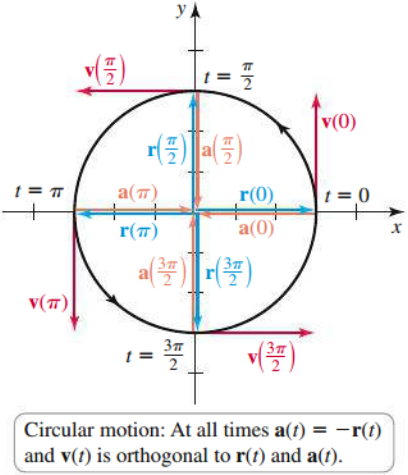
\includegraphics[width=0.35\linewidth]{../images/briggs_14_03/fig14_13}
  \end{flushright}
  \pagebreak

  \begin{thmBox*}[Theorem 14.2: Motion with constant $\abs{\vecr}$]
    Let $\vecr$ describe a path on which $\abs{\vecr}$ is constant (motion on a circle or sphere centered at the origin). Then $\vecr\cdot\vecv=0$, which means the position vector and the velocity vector are orthogonal at all times for which the functions are defined. 
  \end{thmBox*}

  \begin{ex*}[Path on a sphere]
    Consider
      \[\vecr(t)=\bracket{3\cos(t),\,5\sin(t),\,4\cos(t)},\quad\textnormal{for } 0\leq t\leq 2\pi.\]
  \end{ex*}
  \begin{tasks}[after-item-skip=\stretch{1}](1)
    \task Show that an object with this trajectory moves on a sphere and find the radius.
    \task Find the velocity and speed of the above trajectory.
    \task Show that $\vecr(t)=\bracket{5\cos(t),\,5\sin(t),\,5\sin(2t)}$ does not lie on a sphere. How could this function be modified so that it does lie on a sphere?
  \end{tasks}
  \vspace*{\stretch{2}}
  \pagebreak

  \begin{ex*}
    Given $\mathbf a(t)=\bracket{\cos(t),4\sin(t)}$, with an initial velocity $\bracket{\vecu_0,\vecv_0}=\bracket{0,4}$ and an initial position $\bracket{x_0,y_0}=\bracket{5,0}$ where $t\geq 0$, find the velocity and position vector.
  \end{ex*}
  \pagebreak

  \begin{thmBox*}[Summary: Two-Dimensional Motion in a Gravitational Field]
    Consider an object moving in a plane with a horizontal $x$-axis and a vertical $y$-axis, subject only to the force of gravity. Given the initial velocity $\vecv(0)=\bracket{u_0,v_0}$ and the initial position $\vecr(0)=\bracket{x_0,y_0}$, the velocity of the object, for $t\geq 0$, is
      \[\vecv(t)=\bracket{x'(t), y'(t)}=\bracket{u_0,-gt+v_0}\]
    and the position is
      \[\vecr(t)=\bracket{x(t),y(t)}=\bracket{u_0t+x_0,-\frac{1}{2}gt^2+v_0t+y_0}.\]
  \end{thmBox*}

  \begin{ex*}
    Consider a ball with an initial position of $\bracket{x_0,y_0}=\bracket{0,0}\ m$ and an initial velocity of $\bracket{u_0,v_0}=\bracket{25,4}\ m/s$.
  \end{ex*}
  \begin{tasks}[after-item-skip=\stretch{1}](1)
    \task Find the position and velocity of the ball while it is in the air
  \end{tasks}
  \vspace*{\stretch{1}}

%  \pagebreak

  \begin{thmBox*}[Summary: Two-Dimensional Motion]
    Assume an object traveling over horizontal ground, acted on only by the gravitational force, has an initial position $\bracket{x_0,y_0}=\bracket{0,0}$ and initial velocity $\bracket{u_0,v_0}=\bracket{\abs{\vecv_0}\cos\alpha, \abs{\vecv_0}\sin\alpha}$. The trajectory, which is a segment of a parabola, has the following properties.
    \begin{align*}
      \textnormal{time of flight}&= T= \frac{2\abs{\vecv_0}\sin\alpha}{g}\\
      \textnormal{range}&=\frac{\abs{\vecv_0}^2\sin\parens{2\alpha}}{g}\\
      \textnormal{maximum height}&=y\parens{\frac{T}{2}}=\frac{\parens{\abs{\vecv_0}\sin\alpha}^2}{2g}
    \end{align*}
  \end{thmBox*}

  \pagebreak
  \begin{ex*}
    Consider a ball with an initial position of $\bracket{x_0,y_0}=\bracket{0,0}\ m$ and an initial velocity of $\bracket{u_0,v_0}=\bracket{25,4}\ m/s$. Assuming the ground is flat and level:
  \end{ex*}
  \begin{tasks}[after-item-skip=\stretch{1}, resume](1)
    \task How long is the ball in the air?
    \task How far does the ball travel horizontally? 
    \task What is the maximum height that the ball reaches?
  \end{tasks}
  \vspace*{\stretch{1}}
  \pagebreak
  
\end{document}